%%% The main file. It contains definitions of basic parameters and includes all other parts.

%% Settings for single-side (simplex) printing
% Margins: left 40mm, right 25mm, top and bottom 25mm
% (but beware, LaTeX adds 1in implicitly)
\documentclass[12pt,a4paper]{report}
\setlength\textwidth{145mm}
\setlength\textheight{247mm}
\setlength\oddsidemargin{15mm}
\setlength\evensidemargin{15mm}
\setlength\topmargin{0mm}
\setlength\headsep{0mm}
\setlength\headheight{0mm}
% \openright makes the following text appear on a right-hand page
\let\openright=\clearpage

%% Settings for two-sided (duplex) printing
% \documentclass[12pt,a4paper,twoside,openright]{report}
% \setlength\textwidth{145mm}
% \setlength\textheight{247mm}
% \setlength\oddsidemargin{14.2mm}
% \setlength\evensidemargin{0mm}
% \setlength\topmargin{0mm}
% \setlength\headsep{0mm}
% \setlength\headheight{0mm}
% \let\openright=\cleardoublepage

%% Prefer Latin Modern fonts
\usepackage{lmodern}

%% Further useful packages (included in most LaTeX distributions)
\usepackage{amsmath}        % extensions for typesetting of math
\usepackage{amsfonts}       % math fonts
\usepackage{amsthm}         % theorems, definitions, etc.
\usepackage{bbding}         % various symbols (squares, asterisks, scissors, ...)
\usepackage{bm}             % boldface symbols (\bm)
\usepackage{graphicx}       % embedding of pictures
\usepackage{fancyvrb}       % improved verbatim environment
\usepackage{natbib}         % citation style AUTHOR (YEAR), or AUTHOR [NUMBER]
\usepackage[nottoc]{tocbibind} % makes sure that bibliography and the lists
			    % of figures/tables are included in the table
			    % of contents
\usepackage{dcolumn}        % improved alignment of table columns
\usepackage{booktabs}       % improved horizontal lines in tables
\usepackage{paralist}       % improved enumerate and itemize
\usepackage[usenames, table]{xcolor}  % typesetting in color

\usepackage[obeyspaces]{url}

\usepackage[colorinlistoftodos,prependcaption,textsize=tiny]{todonotes}
\usepackage{xargs}
\newcommandx{\unsure}[2][1=]{\todo[linecolor=red,backgroundcolor=red!25,bordercolor=red,#1]{#2}}
\newcommandx{\change}[2][1=]{\todo[linecolor=blue,backgroundcolor=blue!25,bordercolor=blue,#1]{#2}}
\newcommandx{\info}[2][1=]{\todo[linecolor=OliveGreen,backgroundcolor=OliveGreen!25,bordercolor=OliveGreen,#1]{#2}}
\newcommandx{\improvement}[2][1=]{\todo[linecolor=Plum,backgroundcolor=Plum!25,bordercolor=Plum,#1]{#2}}
\newcommandx{\thiswillnotshow}[2][1=]{\todo[disable,#1]{#2}}

\usepackage{enumitem}
\usepackage{usebib}
\usepackage{tikz}

%% Generate PDF/A-2u
\usepackage[a-2u]{pdfx}

%% Character encoding: usually latin2, cp1250 or utf8:
\usepackage[utf8]{inputenc}

\usepackage{hyperref}


%%% Basic information on the thesis

%%% XXX TODO
\title{HexMage}

% Thesis title in English (exactly as in the formal assignment)
\def\ThesisTitle{Using procedural content generation to balance encounters in RPG-like games}

% Author of the thesis
\def\ThesisAuthor{Jakub Arnold}

% Year when the thesis is submitted
\def\YearSubmitted{2017}

% Name of the department or institute, where the work was officially assigned
% (according to the Organizational Structure of MFF UK in English,
% or a full name of a department outside MFF)
\def\Department{Department of Software and Computer Science Education}

% Is it a department (katedra), or an institute (ústav)?
\def\DeptType{Department}

% Thesis supervisor: name, surname and titles
\def\Supervisor{Mgr. Jakub Gemrot}

% Supervisor's department (again according to Organizational structure of MFF)
\def\SupervisorsDepartment{Department of Software and Computer Science Education}

% Study programme and specialization
\def\StudyProgramme{Computer Science}
\def\StudyBranch{Programming and Software Systems}

% An optional dedication: you can thank whomever you wish (your supervisor,
% consultant, a person who lent the software, etc.)
\def\Dedication{%
Dedication.
}

% Abstract (recommended length around 80-200 words; this is not a copy of your thesis assignment!)
\def\Abstract{%
Procedural content generation (PCG) is mostly examined in the context of
map/environment creation, rather than generating the actual game characters.
The goal of this thesis is to design a turn-based RPG-like game with perfect information
for which we can generate balanced encounters. The game consists of a hex-based arena
in which two teams fight. Each team consists of a few player controller characters
with unique abilities. We generate the attributes of these abilities in order
to make the encounter balanced. We will also build an AI that
can be used to automatically play-test the PCG algorithm. The goal is to generate an equally
strong, but different opponent.}

% 3 to 5 keywords (recommended), each enclosed in curly braces
\def\Keywords{%
{video games} {encounter balancing} {hex arena} {rpg elements}
}

%% The hyperref package for clickable links in PDF and also for storing
%% metadata to PDF (including the table of contents).
%% Most settings are pre-set by the pdfx package.
\hypersetup{unicode}
\hypersetup{breaklinks=true}

% Definitions of macros (see description inside)
%%% This file contains definitions of various useful macros and environments %%%
%%% Please add more macros here instead of cluttering other files with them. %%%

%%% Minor tweaks of style

% These macros employ a little dirty trick to convince LaTeX to typeset
% chapter headings sanely, without lots of empty space above them.
% Feel free to ignore.
\makeatletter
\def\@makechapterhead#1{
  {\parindent \z@ \raggedright \normalfont
   \Huge\bfseries \thechapter. #1
   \par\nobreak
   \vskip 20\p@
}}
\def\@makeschapterhead#1{
  {\parindent \z@ \raggedright \normalfont
   \Huge\bfseries #1
   \par\nobreak
   \vskip 20\p@
}}
\makeatother

% This macro defines a chapter, which is not numbered, but is included
% in the table of contents.
\def\chapwithtoc#1{
\chapter*{#1}
\addcontentsline{toc}{chapter}{#1}
}

% Draw black "slugs" whenever a line overflows, so that we can spot it easily.
\overfullrule=1mm

%%% Macros for definitions, theorems, claims, examples, ... (requires amsthm package)

\theoremstyle{plain}
\newtheorem{thm}{Theorem}
\newtheorem{lemma}[thm]{Lemma}
\newtheorem{claim}[thm]{Claim}

\theoremstyle{plain}
\newtheorem{defn}{Definition}

\theoremstyle{remark}
\newtheorem*{cor}{Corollary}
\newtheorem*{rem}{Remark}
\newtheorem*{example}{Example}

%%% An environment for proofs

%%% FIXME %%% \newenvironment{proof}{
%%% FIXME %%%   \par\medskip\noindent
%%% FIXME %%%   \textit{Proof}.
%%% FIXME %%% }{
%%% FIXME %%% \newline
%%% FIXME %%% \rightline{$\square$}  % or \SquareCastShadowBottomRight from bbding package
%%% FIXME %%% }

%%% An environment for typesetting of program code and input/output
%%% of programs. (Requires the fancyvrb package -- fancy verbatim.)

\DefineVerbatimEnvironment{code}{Verbatim}{fontsize=\small, frame=single}

%%% The field of all real and natural numbers
\newcommand{\R}{\mathbb{R}}
\newcommand{\N}{\mathbb{N}}

%%% Useful operators for statistics and probability
\DeclareMathOperator{\pr}{\textsf{P}}
\DeclareMathOperator{\E}{\textsf{E}\,}
\DeclareMathOperator{\var}{\textrm{var}}
\DeclareMathOperator{\sd}{\textrm{sd}}

%%% Transposition of a vector/matrix
\newcommand{\T}[1]{#1^\top}

%%% Various math goodies
\newcommand{\goto}{\rightarrow}
\newcommand{\gotop}{\stackrel{P}{\longrightarrow}}
\newcommand{\maon}[1]{o(n^{#1})}
\newcommand{\abs}[1]{\left|{#1}\right|}
\newcommand{\dint}{\int_0^\tau\!\!\int_0^\tau}
\newcommand{\isqr}[1]{\frac{1}{\sqrt{#1}}}

%%% Various table goodies
\newcommand{\pulrad}[1]{\raisebox{1.5ex}[0pt]{#1}}
\newcommand{\mc}[1]{\multicolumn{1}{c}{#1}}


% Title page and various mandatory informational pages
\begin{document}
%%% Title page of the thesis and other mandatory pages

%%% Title page of the thesis

\pagestyle{empty}
\hypersetup{pageanchor=false}
\begin{center}

\centerline{\mbox{
\includegraphics[width=166mm]{img/logo-en.pdf}}}

\vspace{-8mm}
\vfill

{\bf\Large BACHELOR THESIS}

\vfill

{\LARGE\ThesisAuthor}

\vspace{15mm}

{\LARGE\bfseries\ThesisTitle}

\vfill

\Department

\vfill

\begin{tabular}{rl}

Supervisor of the bachelor thesis: & \Supervisor \\
\noalign{\vspace{2mm}}
Study programme: & \StudyProgramme \\
\noalign{\vspace{2mm}}
Study branch: & \StudyBranch \\
\end{tabular}

\vfill

% Zde doplňte rok
Prague \YearSubmitted

\end{center}

\newpage

%%% Here should be a bound sheet included -- a signed copy of the "bachelor
%%% thesis assignment". This assignment is NOT a part of the electronic
%%% version of the thesis. DO NOT SCAN.

%%% A page with a solemn declaration to the bachelor thesis

\openright
\hypersetup{pageanchor=true}
\pagestyle{plain}
\pagenumbering{roman}
\vglue 0pt plus 1fill

\noindent
I declare that I carried out this bachelor thesis independently, and only with the cited
sources, literature and other professional sources.

\medskip\noindent
I understand that my work relates to the rights and obligations under the Act No.~121/2000 Sb.,
the Copyright Act, as amended, in particular the fact that the Charles
University has the right to conclude a license agreement on the use of this
work as a school work pursuant to Section 60 subsection 1 of the Copyright Act.

\vspace{10mm}

\hbox{\hbox to 0.5\hsize{%
In ........ date ............	% FIXME!
\hss}\hbox to 0.5\hsize{%
signature of the author
\hss}}

\vspace{20mm}
\newpage

%%% Mandatory information page of the thesis

\openright

\vbox to 0.5\vsize{
\setlength\parindent{0mm}
\setlength\parskip{5mm}

Title:
\ThesisTitle

Author:
\ThesisAuthor

\DeptType:
\Department

Supervisor:
\Supervisor, \SupervisorsDepartment

Abstract:
\Abstract

Keywords:
\Keywords

\vss}

\newpage

%%% Dedication

\openright

\noindent
\Dedication

\newpage

\openright
\pagestyle{plain}
\pagenumbering{arabic}
\setcounter{page}{1}


%%% A page with automatically generated table of contents of the bachelor thesis

\tableofcontents

%%% Each chapter is kept in a separate file
\chapwithtoc{Introduction}

An increasing number of computer games is using procedural content generation
(PCG) as one of their core mechanics. This is in different contexts, most
commonly for generating new levels (e.g. \citet{diablo}). \todo{zobrazovat nazev a ne autora} Occasionally games
even generate player collectible items (e.g. \citet{borderlands}). However,
there has not been much research on the use of procedural generation for
balancing encounters in RPG games. By this we mean procedurally generating
enemies that can be defeated by the player, but pose a challenge. A crucial
criteria here is that the balance is not simply achieved by creating the enemy
as an exact clone of the player, but rather explore the search-space to find an
enemy that is not only balanced, but also different from the player.

One particular application for this kind of PCG is automatic difficulty
adjustments based on the player's skill. Another possible use could be
automatic generation of new and unique enemies based on given constraints,
which is the approach we chose in this thesis.

We have created a custom game with mechanics that are simple enough to simulate
quickly, yet flexible enough to represent a large search space. There are two
teams that fight in a hexagonal arena, each consists of a small number of
player controlled characters (mages), and each mage has a small number of
abilities. In each turn the player has control over one of his characters, and
both move around the map and cast spells, in any order he wishes. The only
limit is the number of action points the character has available, which are
consumed both by movement and ability usage. The side that first eliminates the
opposing team wins.

All information is visible to all players, and all actions are completely
deterministic. There is no time limit for the player action, which means the
player could theoretically calculate a perfect move given enough time.

The goal of this thesis is to explore PCG options for balancing encounters in
turn-based RPG-like games. We design a simple game with flexible mechanics, and
build an AI that can be used to approximate the player. We then use evolution strategies
to generate opponents of just the right difficulty for the given player team, using AI vs
AI combat as a fitness function.

\subsection*{Organization}

In Chapter 1 we begin by defining the scope of the work, our general approach,
and list related work. Chapter 2 follows by exploring our game mechanics in
detail and explaining the choices behind them. Next in Chapter 3 we will go
over our different choices for implementing the AI.

Chapter 4 describes our approach to generating the encounters, with the expriments
described in Chapter 5 and a conclusion in Chapter 6. Lastly, the Appendix contains
programmer documentation with implementation details.

% \part{Analysis}
\chapter{Problem Definition}

\section{Game types}

\section{Types of PCG currently being used}

\section{Our game}

- game that can generalize to real life scenarios
- simple mechanics that are representative
- fast to simulate


Two teams fight on a hexagonal map (\emph{arena}) of small size (radius of
5-10 hexes). Each team consists of a small number of player controller
characters (\emph{mages} for short), and each mage has a small number of
\emph{abilities}, \emph{health}, and \emph{action points}. Players take turns, during
which each player has control over one of his mages. The player can issue
commands to move around the arena and use abilities. Both movement and ability
usage costs action points, which are restored at the end of the turn.  Moving
one hex costs one action point. The cost of using an ability varies, and is one
of the parameters that we optimize for when looking for a balanaced game. An
ability can also have a \emph{cooldown}, which prevents repeated usage for a
given number of turns \todo{znovu rozlisovat turn}. Note that the cooldown can
be zero, which means the ability can be used multiple times per turn
\todo{turn}.

\missingfigure{obrazek areny?}

Abilities can do direct damage to an enemy mage, apply a \emph{debuff} (causing
damage and decreasing action points over time), and create an area of effect
(\emph{AOE}) debuff that spans multiple hexes in the arena. Both the debuffs and
AOEs are applied at the end of each turn \todo{rozlisovat turn maga a turn hry
(round?)}, which happens after both players finish playing all their mages.
Both debuffs and AOEs also have a lifetime, which specifies how many turns
\todo{znova turn} the effect lasts.

% \part{Implementation}
\chapter{Game Rules and Mechanics}
\label{chapter02}

Two teams fight on a hexagonal map (\emph{arena}) of small size (radius of
5--10 hexes, see \autoref{fig:arena}). The map contains empty hexes and walls.
Each team consists of a small number of player controller
characters (\emph{mages} for short), and each mage has a small number of
\emph{abilities}, \emph{health}, and \emph{action points}. Players take turns, during
which each player has control over one of his mages. The player can issue
commands to move around the arena and use abilities. Mages can only walk on empty hexes
and cannot cast through walls.

There is also an important distinction between a \emph{turn} and a \emph{round}.
A turn means playing all the actions a single mage can do with his action points,
and ends when the player decides he is finished playing with that one single character.
A round ends when all of the characters have played their turn, and it is at that point
when debuffs, AOEs, cooldowns and action points are re-calculated (see below).

Both movement and ability usage costs action points, which are restored at the
end of the round. Moving one hex costs one action point. The cost of using an
ability varies, and is one of the parameters that we optimize for when looking
for a balanaced game. An ability can also have a \emph{cooldown}, which
prevents repeated usage for a given number of rounds. Note that the cooldown
can be zero, which means the ability can be used multiple times per turn.
Abilities also have limited range, which supports positional gameplay.

Abilities can do direct damage to an enemy mage, apply a \emph{debuff} (causing
damage and decreasing action points over time), and create an area of effect
(\emph{AOE}) debuff that spans multiple hexes in the arena. Both the debuffs and
AOEs are applied at the end of each round. Both debuffs and AOEs also have a lifetime,
which specifies how many rounds the effect lasts.

The motivation for having cooldowns is that it allows us to generate powerful
abilities that don't necessarily take up the whole turn of the player by costing
a lot of action points. If the ability is cheap, but has a large cooldown, it can
serve a strategic purpose, as the player might want to prepare his position in order
to use the ability when the cooldown wears off. AOE abilities also improve positional
gameplay, as they can be used to force the enemy player to move out of position.

\begin{figure}[h]
	\centering
	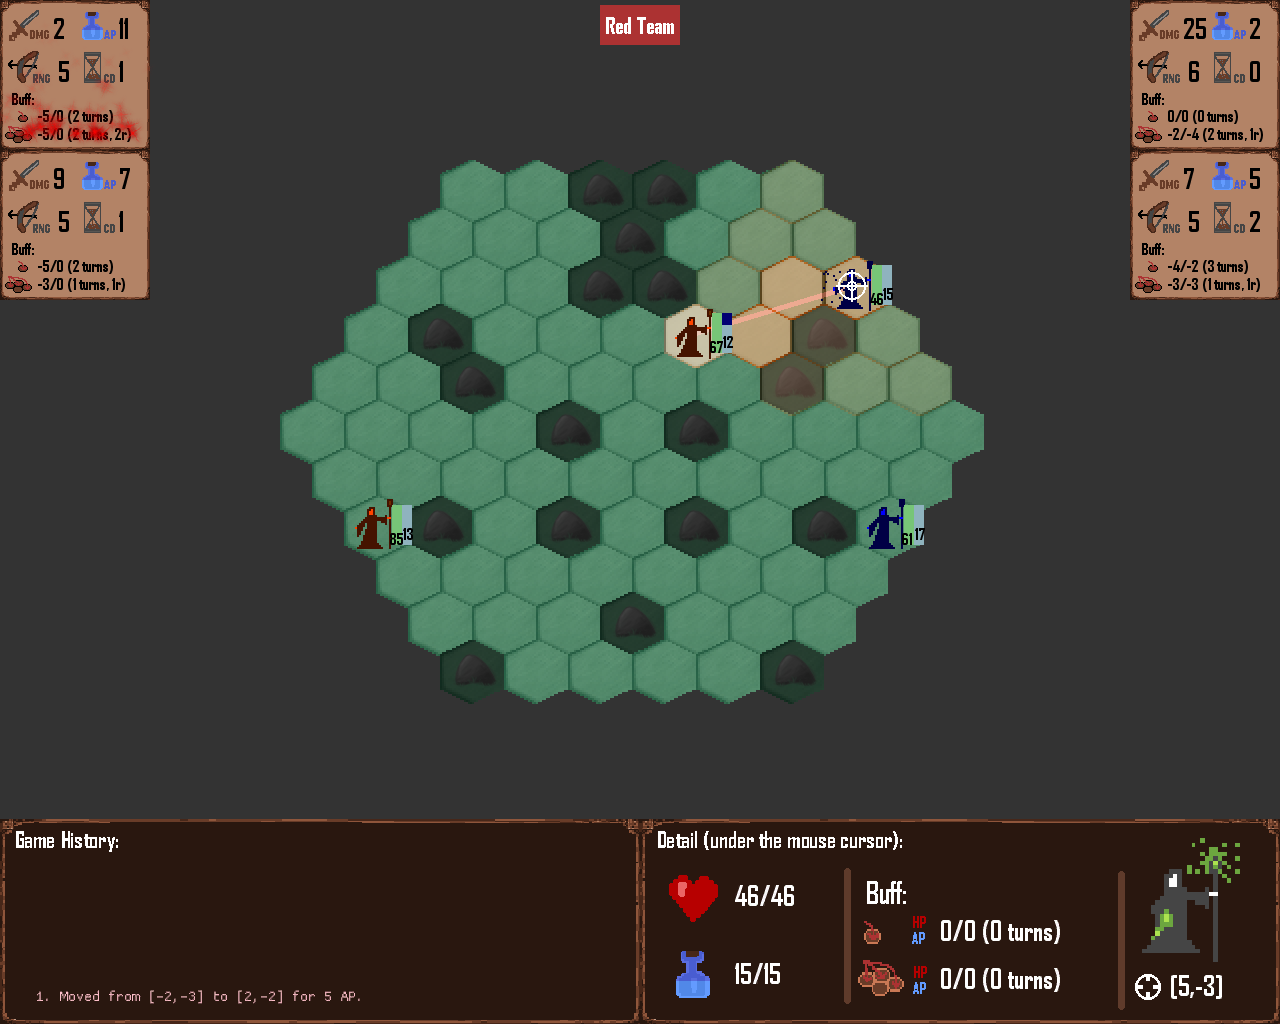
\includegraphics[width=0.95\textwidth]{img/arena.png}
	\caption{User interface of the HexMage game, featuring a 2v2 game. The red player currently has a spell selected and is targeting one of the blue player's mages.}
	\label{fig:arena}
\end{figure}


\section{Simulator}

Part of our game is a simulator that can be used as a library and encapsulates
all of the game rules and mechanics. This is then used by both the AI and the
PCG algorithm and can thus be run separately from the main game. The game is
internally represented by a \emph{state} object, and all of the possible player
actions are encapsulated by an \emph{action} object.  Playing the game through
the library then simply becomes a matter of applying a state transition
function $f: (\text{state}, \text{action}) \rightarrow \text{state}$.

Here's a list of all possible actions at an arbitrary state:

\begin{description}
\item [AbilityUse] Use an ability targeting an enemy that is already in range.
\item [Move] Move the current mage to a different hex on the map.
\item [EndTurn] Finish the current turn.
\item [DefensiveMove] Serves the same purpose as \emph{Move}, but carries an
additional information in the sense that \emph{DefensiveMove} can only be
the last action of the turn.
\item [AttackMove] Combines the \emph{Move} and \emph{AbilityUse} actions into one.
\item [NullAction] Doesn't do anything and is mostly used as a placeholder in cases no action is possible.
\end{description}

The simulator also verifies that no invalid actions are applied through a
thorough list of invariant checks. These are automatically turned off in a
release build to make the simulator run as fast as possible.

The simulator is also built to be high performance and can easily run hundreds
of thousands to millions of actions per second on a consumer-grade PC\@.
The state object is split into two parts, one that handles the
general immutable information that doesn't change as the game progresses (i.e.\
max hitpoints, ability definitions, etc.), and one that handles all of the
mutable data, such as current hitpoints, current positions on the map, etc.
This allowed us to make state copies very fast as well, running only at a few
microseconds per copy.

\chapter{Generating Encounters}

We approach generating encounters as a search based problems with two
different approaches, Simulated Annealing and Evolution Strategies. (\todo{reference})

To make the search algorithms as general as possible, we serialize our
internal game representation into a single vector of normalized floating
point values (DNA). The algorithm then doesn't need to understand our game
mechanics and restriction, and can be applied to different configurations of
the game independently.

To avoid balancing via specific attributes, one can simply remove them from
the serialization/deserialization routines that transform the game setup into
the DNA vector, without altering any of the logic for balancing encounters.

In the case of our experiments, we chose to stick with 2v2 games on a fixed map,
where each mage has only two abilities. This was chosen both with respect to our
questionnaire, and running time of the algorithms. Choosing a larger team setup or
a bigger map (or many different maps) would be difficult for the participants,
and would also take much longer to compute our experimental data.

\missingfigure{mapa}

- popsat jak funguje reprezentace DNA

\section{Simulated Annealing and Evolution Strategies}

Our initial implementation of generating the encounters was using Simulated
Annealing (\todo{reference}). However, we had difficulty converging to good
results \todo{fuj, napsat jinak}.

As a result, we ran an experiment to sample the search space at roughly 20 million
different points, and measured the change in fitness in the neighbourhood of each point.
We found that in each point's neighbourhood, there are roughly 5 times more points that have
worse fitness than the ones that are an improvement over the current point. We also found that
most of these downward changes were much steeper between 4-7x than the improving points.

Our suspicion is that this is the main cause of failure of Simmulated Annealing, which simply
fails to find the upward slope.

For this reason we chose to try another approach, specificially Evolution Strategies (\todo{reference})

\section{Choice of the Fitness Function}

In order to evaluate the balance of a matchup, we came up with the following fitness function.

\todo{chybi popis}

During the experiment we encountered multiple ways ES tried to exploit the game
mechanics to maximize the balance fitness function in ways that were
undesirable. One example being when the resulting games end up being short as
the algorithm generates mages with lots of AOE abilities that cover the whole
map in the first turn, resulting in immediate death of all characters.

We balance this by introducing an additional fitness function for game length
in the form of a cumulative normal distribution with $\sigma = 10$ and $\mu =
3$.\unsure{overit jestli to tak fakt je}.  This prevents ES from moving towards
short games.

\chapter{Generating Encounters}
\label{chapter04}

There are many possible attributes that can be generated. We could change the size of each team,
the number of abilities of each mage, starting positions of the map, or even change the positions of the walls.

\section{Reducing the Scope of the Problem}

We chose to reduce the scope by creating a small fixed map on which all encounters will be played and balanced.
We also fix the team size of both teams to 2 mages, and each mage to 2 abilities. While this significantly reduces
the possibilities to achieve balance, there are still a lot of parameters that can be tweaked, as described in the next section.

We also put lower and upper bounds on most of the numeric values of attributes of mages and their abilities. See attached programmer documentation in the \autoref{chap:prog-doc} for more details about how attributes are represented.

\section{Approach}

We approach generating encounters as a search based problems with two different
approaches, Simulated Annealing \citep{ai-modern} and Evolution Strategies
\citep{evolution-strategies}.

To make the search algorithms as general as possible, we serialize our
internal game representation into a single vector of normalized floating
point values (DNA). The algorithm then does not need to understand our game
mechanics and restriction, and can be applied to different configurations of
the game independently.

To avoid balancing via specific attributes, one can simply remove them from
the serialization/deserialization routines that transform the game setup into
the DNA vector, without altering any of the logic for balancing encounters.

In the case of our experiments, we chose to stick with 2v2 games on a fixed map,
where each mage has only two abilities. This was chosen both with respect to our
questionnaire, and running time of the algorithms. Choosing a larger team setup or
a bigger map (or many different maps) would be difficult for the participants,
and would also take much longer to compute our experimental data.

Taking these restrictions into mind, the DNA would then take up $96$ floating point values,
specifically: $$2 \text{ Teams} \times 2 \text{ Mages} \times ( HP + AP + 2 \times \text{AbilitySize}) = 96$$ since $\text{Ability Size} = 11$ as we need to serialize damage, cost, range, cooldown,
debuff (HP damage, AP damage, lifetime), and AOE (debuff + lifetime).

\todo{popsat hillclimbing}

\section{Simulated Annealing}

Our initial implementation of generating the encounters was using Simulated
Annealing \citep{ai-modern}. Simulated annealing works similar to a hill climbing algorithm, except
that instead of always picking the best neighbour, we use a probability distribution.
Neighbours with better fitness have a higher probability, but we might still take a path
downhill. The amount of randomness is controlled by an external variable called temperature (or energy).
As the algorithm progresses, the temperature is slowly reduced and thus allows it to converge.
The main advantage over hill climbing is that simulated annealing does not immediately get stuck in a local optima,
as there is always a chance it will move to a state with lower fitness value.

However, we had difficulty getting good results and the algorithm
almost never converged. As a result, we ran an experiment to sample the search space at roughly 20
million different points, and measured the change in fitness in the
neighbourhood of each point. We found that in each point's neighbourhood,
there are roughly 5 times more points that have worse fitness than the ones
that are an improvement over the current point. We also found that most of
these downward changes were much steeper between 4--7x than the improving
points. Our suspicion is that this is the main cause of failure of
Simmulated Annealing, which simply fails to find the upward slope.

\section{Evolution Strategies}

For this reason we chose to try another approach, specificially Evolution
Strategies (ES) \citep{evolution-strategies}. ES works by taking a random sample of the
neighbourhood of the current value, evaluating the fitness of each of the neighbours, and
moving to a state that is the weighted average of the neighbours with respect to their fitness.
This process is iterated until a state with suitable fitness value is found. In our experiments
we have found this approach to consistently converge much faster than simulated annealing.

ES also yields itself to easy parallelization, especially if the evaluation of the fitness
function is complicated. Since all of the neighbouring samples are completely independent,
they can be evaluated completely in parallel.

\section{Choice of the Fitness Function}

In order to evaluate the balance of a matchup, we evaluated the following three
criteria:

\begin{description}
\item [Balance] Unsurprisingly, part of the fitness function is comparing the
  strength of both teams against each other.  We consider games that end in a
    draw balanced.  If the game doesn't end in a draw, we measure the remaining
    HP percentage of the winner, and the lower it is, the more balanced the
    game was.
\item [Game length] We also put an interval restriction on game length. Ideally
  we'd want the game to last at least 2 rounds.
\item [Team difference] Lastly, since we don't to create balance by making both
  teams identical, we added a third criteria that measures the difference of
    both teams.
\end{description}

The combined fitness function is calculated as the average of the three.
See \hyperref[fig:converging-es]{Figure 4.1} for an example
plot of how the fitness function converges using Evolution Strategies.
It is worth noting here that evaluating the fitness function (the \emph{Balance}
part specifically) is computationally intensive, as it requires the whole game
to be played out till the end. We also do this evaluation using an ensemble average of multiple different AIs.
Specifically, we use both the Rule based AI and MCTS in the \emph{Balance} playout and take their average.
This helps assure that the game is balanced despite multiple playstyles, as both the Rule based AI and MCTS
play differently (see \hyperref[tab:winrates]{Table 5.1} for their comparison). You can see how the fitness function
converges in \hyperref[fig:converging-es]{Figure 4.1}.

\begin{figure}
	\centering
	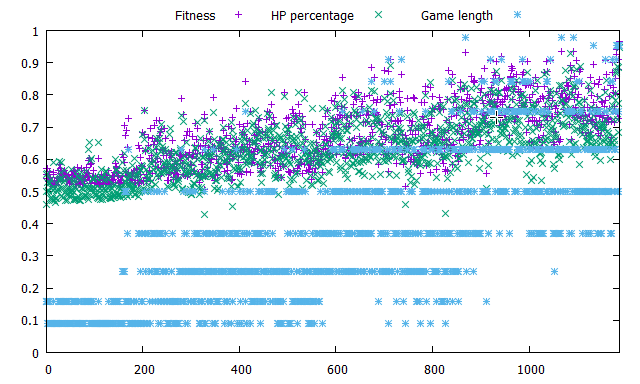
\includegraphics[width=0.75\textwidth]{img/converging-es.png}
	\caption{An exmple of a how the combined fitness function converges over rougly 1200 iterations. Green dots represent the \emph{Balance} fitness measuring HP percentage left at the end of the game, blue dots represent game length, and purple is the combined fitness. We're not showing team difference data points as in this plot.}
	\label{fig:converging-es}	
\end{figure}

\section{Remarks}

During the experiment we encountered multiple ways ES tried to exploit the
game mechanics to maximize the balance fitness function in ways that were
undesirable. One example being when the resulting games end up being short
as the algorithm generates mages with lots of AOE abilities that cover the
whole map in the first turn, resulting in immediate death of all characters.

We balance this by introducing an additional fitness function for game length
in the form of a cumulative normal distribution with mean around $10$ turns.

Lastly, the team difference is measured as an euclidean distance between the DNA
vectors of each team. Again, we use a cumulative normal distribution to put a lower
bound on the team difference.

\chapter{Experiments}
\label{chapter05}

\section{Participants}

The participants were all computer science students. All of them had at least
some experience with computer games, and were presented the mechanics of HexMage
before conducting the experiment.

\section{Experiment Design}

The goal of the experiment is to measure two things. One, if the generated
encounters are actually balanced. And two, if the AI is strong enough to pose a
challenge to the player. We will measure the overall winrate of the players,
and also compare how the AI did in games the player considered balanced.

The experiment consists of 20 different games of HexMage. All of the games are
played on the same map that was hand-designed beforehand. This was to allow the
participants to better get familiar with the game and think ahead. The games
are structured so that each player has 2 mages, each with 2 abilities. This was
to reduce the cognitive overhead for the participants and allow them to more easily
adjust to the 20 completely different scenarios.

The first 10 of the 20 games had the player team hand designed, and the
opponent (played by the AI) generated with our PCG algorithm. The remaining 10
games had both teams generated with no manual tweaks or changes. Having some of
the games hand designed allows us to show that the PCG algorithm can balance
against constraints that aren't completely random. A hand designed team might
have features that are rare in the search space. All of the games are played
against the MCTS based AI\@.

\section{Results}

\missingfigure{korelacni matice}
\missingfigure{grafy}

The results show that most participants consider our MCTS AI to be strong
enough to provide a challengem which is also proven by the 40\% winrate of
the participants. \todo{aktualizovat cisla}

Given the number of played games \todo{overit, ze jich mame dost} we can
rule out the AI having a better setup in most of the scenarios. Based on the
results, around 35\% \todo{aktualizovat cisla} of the games were balanced,
which means in the resulting 65\% one of the players had an advantage.

We consider this result to be positive as the games were generated without
any human intervention and weren't altered before running the experiment.
\todo{link na appendinx s instrukcema na pregenerovani experimentu}

Considering that 35\% of the generated games are balanced, this would allow
the algorithm to be used offline as is to aid design of game levels with
some manual checking of the resulting games.

If one were to design the encounter completely from scratch to be balanced,
it would be very difficult given the number of variables that need to be
optimized.

\section{TODO}

\begin{description}[align=right,labelwidth=3cm]
\item bud zminit ze by to slo delat online s nejaky additional checkem
\item nebo zlepsit fitness aby vyresila patologicke pripady z experimentu?
\end{description}


\chapter{Conclusion and discussion of the results}

\chapter{Conclusion}
\label{chapter06}

We have designed and developed a working game with a simulator, developed multiple
AI bots, built an algorithm for generating balanced encounters and tested everything
in a number of experiments.

Our experimental findings confirm that search based procedural generation
is a viable solution for balancing encounters. While we didn't achieve perfect
accuracy in generating balanced results, our participants considered around $60\%$
of the games to be balanced. This is confirmed by our win rate results, where $75\%$
of the games were not completely won/lost by the players. After manually checking the remaining
$25\%$ we found that one of the games was actually possible to win, which would raise the accuracy
to $80\%$. We think of this as a success, as the games were generated with no human input or modifications to the data.

Our MCTS AI also showed to be working very well, as it decisively defeated both the Random, and the Rule based AI.
It also did well against the human players in the experiment, reaching $62\%$ win rate, and having around $75\%$ of the
games be voted as \emph{smart} and \emph{challenging} by the participants.

\section{Future work}

There are many opportunities for future work. One would be to develop a more sophisticated fitness function that
takes into account problems mentioned in \hyperref[chapter05]{Chapter 5}. Team sizes could also be adjusted and allow changing the number of mages in a team and the number of their abilities as part of the evolution. Lastly, one could consider balancing regardless of the map the game is going to be played on, and generate the team such that it can adjust to different scenarios.

We also restricted a few mechanics in order to help things converge faster. For example, healing spells are not allowed in our simulator. Enabling them however runs the risk of games taking much longer, and they might not even finish if the amount of healing is greater than the amount of damage. One could also consider allowing AOE abilities to be targeted on the ground, and not just on the enemy mages. While this is possible in many of the popular games, it greatly increases the number of possible actions in each state where an AOE ability is available.


%%% Bibliography
%%% Bibliography (literature used as a source)
%%%
%%% We employ bibTeX to construct the bibliography. It processes
%%% citations in the text (e.g., the \cite{...} macro) and looks up
%%% relevant entries in the bibliography.bib file.
%%%
%%% The \bibliographystyle command selects, which style will be used
%%% for references from the text. The argument in curly brackets is
%%% the name of the corresponding style file (*.bst). Both styles
%%% mentioned in this template are included in LaTeX distributions.

\bibliographystyle{plain}    %% Author (year)
% \bibliographystyle{unsrt}     %% [number]

\renewcommand{\bibname}{Bibliography}

%%% Generate the bibliography. Beware that if you cited no works,
%%% the empty list will be omitted completely.

\bibliography{bibliography}

%%% If case you prefer to write the bibliography manually (without bibTeX),
%%% you can use the following. Please follow the ISO 690 standard and
%%% citation conventions of your field of research.

% \begin{thebibliography}{99}
%
% \bibitem{lamport94}
%   {\sc Lamport,} Leslie.
%   \emph{\LaTeX: A Document Preparation System}.
%   2nd edition.
%   Massachusetts: Addison Wesley, 1994.
%   ISBN 0-201-52983-1.
%
% \end{thebibliography}


%%% Figures used in the thesis (consider if this is needed)
\listoffigures

%%% Tables used in the thesis (consider if this is needed)
%%% In mathematical theses, it could be better to move the list of tables to the beginning of the thesis.
\listoftables

%%% Abbreviations used in the thesis, if any, including their explanation
%%% In mathematical theses, it could be better to move the list of abbreviations to the beginning of the thesis.
\chapwithtoc{Abbreviations and Terminology}

\begin{description}
	\item[MCTS] Monte-Carlo Tree Search
	\item[UCT] Upper Confidence Bound for Trees
	\item[UCB] Upper Confidence Bound for the multi-armed bandit problem.
	
	\item[Winrate] The percentage of games a player has won in a set number of games. For example winning $3$ out of $10$ games gives a $33\%$ winrate
	
	\item[Turn] Playing a single mage until the \verb|EndTurn| action is considered a \emph{turn}. Each mage gets to play one turn within a single round.
	
	\item[Round] When all mages play their turn it is considered one round. Debuffs and AOEs are calculated at the end of each round, and their lifetime is decreased.
	
	\item[Mage] A player or AI controller character.
	
	\item[Damage] The effect of reducing health of a character. Ability with $5$ damage reduces the health of the target by $5$.
	
	\item[Action point] A resource which can be spent both on movement and ability usage. Moving one hex costs one action point, and using an ability costs as many as is defined in the ability's description.
	
	\item[Cooldown] If an ability has an associated \emph{cooldown}, using it disables the ability for the number of rounds as specified by the cooldown attribute.

	\item[Debuff] A temporary effect of an ability which causes the target to low health and action points for a given amount of time. Debuffs have a defined lifetime, which is the number of rounds they last.
	
	\item[AOE] Area of Effect debuffs are similar to \emph{Debuffs}, but they're placed on the ground instead of the targeted mage. AOEs have a defined radius which they affect, and they also have an associated debuff which is applied to a mage standing within the radius at the end of a round.
\end{description}


%%% Attachments to the bachelor thesis, if any. Each attachment must be
%%% referred to at least once from the text of the thesis. Attachments
%%% are numbered.
%%%
%%% The printed version should preferably contain attachments, which can be
%%% read (additional tables and charts, supplementary text, examples of
%%% program output, etc.). The electronic version is more suited for attachments
%%% which will likely be used in an electronic form rather than read (program
%%% source code, data files, interactive charts, etc.). Electronic attachments
%%% should be uploaded to SIS and optionally also included in the thesis on a~CD/DVD.
%%% Allowed file formats are specified in provision of the rector no. 23/2016.
\chapwithtoc{Attachments}

\appendix


\chapter{File formats}
\label{file-formats}

\section{DNA file format}
\label{dna-format}

The DNA vectors are scored in simple text files. The format is as follows:

\begin{itemize}
	\item Each team is stored on a separate line.
	\item The line first contains two numbers, one for the number of mages in a team, and one for the number of abilities of each mage.
	\item Then follows the serialized vector for each mage in the order the mages were defined.
	\item Each mage is stored as his health, action points, and a list of abilities.
	\item Each ability is stored as damage, cost, range, cooldown, debuff, AOE.
	\item Debuff is stored as damage, action point damage and lifetime.
	\item AOE is stored as radius and the effect as if it was a debuff.
\end{itemize}

A reference implementation is in the \path{GenomeLoader.cs} file which contains both serialization and deserialization. Note that the starting positions of the mages are not stored in their DNA, as that information an attribute of the map on which the game is played. See \hyperref[map-format]{the Map file format section} for more details.

We also have an alternative file format for the DNA which can be seen in

\section{Map File Format}
\label{map-format}

The map is stored in a plain JSON file \citep{json}. An example can be found in the \path{data/map.json} file. The file defines the size of the map, whether each hex contains a wall or is empty, and the starting positions of each team. It is important to note that although there can be any number of starting positions on a given map, the team size must not exceed the number of starting positions. If the user tries to start a game with larger teams than the number of starting positions, the program will detect the error and not start the game.


\chapter{User Documentation}

\section{System Requirements}

All of the code is written for \Csh 6.0. The \path{HexMage.GUI} project runs on Windows under .NET framework 4.5 (or newer). It also requires up to date graphics drivers, and optionally audio drivers when running with \texttt{--EnableAudio=true}. The experiments in \path{HexMage.Benchmarks} can be run on Linux under a recent version of Mono (tested on 4.x). See \autoref{sec:compilation} for more detailed instructions on how to compile and run the project.

\section{Generating Experiment Data}

The data for our survey are under the \path{data/manual-teams} directory. Each file represents a single team for which a suitable opponent will be generated by our algorithm. Any number of files can be added.

In order to generate the data for the experiment, simply run the \path{HexMage.Benchmarks.exe} program with no command line arguments (preferably in Release mode) and everything will be generated automatically. The results are stored under \path{data/questionnaire} in separate files in the DNA file format \autoref{dna-format}. Generating the data takes around 1 hour on Intel i7-5820k Processor \citep{intel-ark}. We've disabled parallelization in order to make the data generation deterministic and the whole experiment reproducible. An initial seed is defined under \verb|Constants.RandomSeed| and is used by all of the internal random number generators. Parallel execution can be re-enabled by defining a compile time \verb|PARALLEL| constant.

\section{Running the Experiment}

Running the \path{HexMage.GUI.exe} program will run the experiment by default. It loads the data from \path{data/questionnaire} and presents a list of the required games on the main screen (see \autoref{fig:questionnaire}). The state of the questionnaire is maintained in the files themselves. Specifically, finished games will be renamed to have a \path{.done} extension. This allows the user to resume at any point in time, and also makes it easy to revert back to an initial state if something goes wrong. Pressing \verb|Ctrl-Q| will reset all of the games to unplayed state. This is meant mostly for debugging.

The next game can be started by pressing \verb|Spacebar|, which immediately picks the next game on the list and loads it. After the game is finished, the questionnaire is opened in the default browser and the game identifier is pre-filled (we used Google Forms). The form itself is configured in \verb|QuestionnaireScene.cs|. After the user finishes playing the game, they should quit the program and re-launch it to proceed to the next game. We did this for stability purposes since the questionnaire was run remotely and we had no way to assist the user in case of errors.

We also provide the exact ZIP file we used to run the experiment with all of the generated games to make it easy to reproduce the results without having to run the encounter generation script.

\begin{figure}[h]
	\centering
	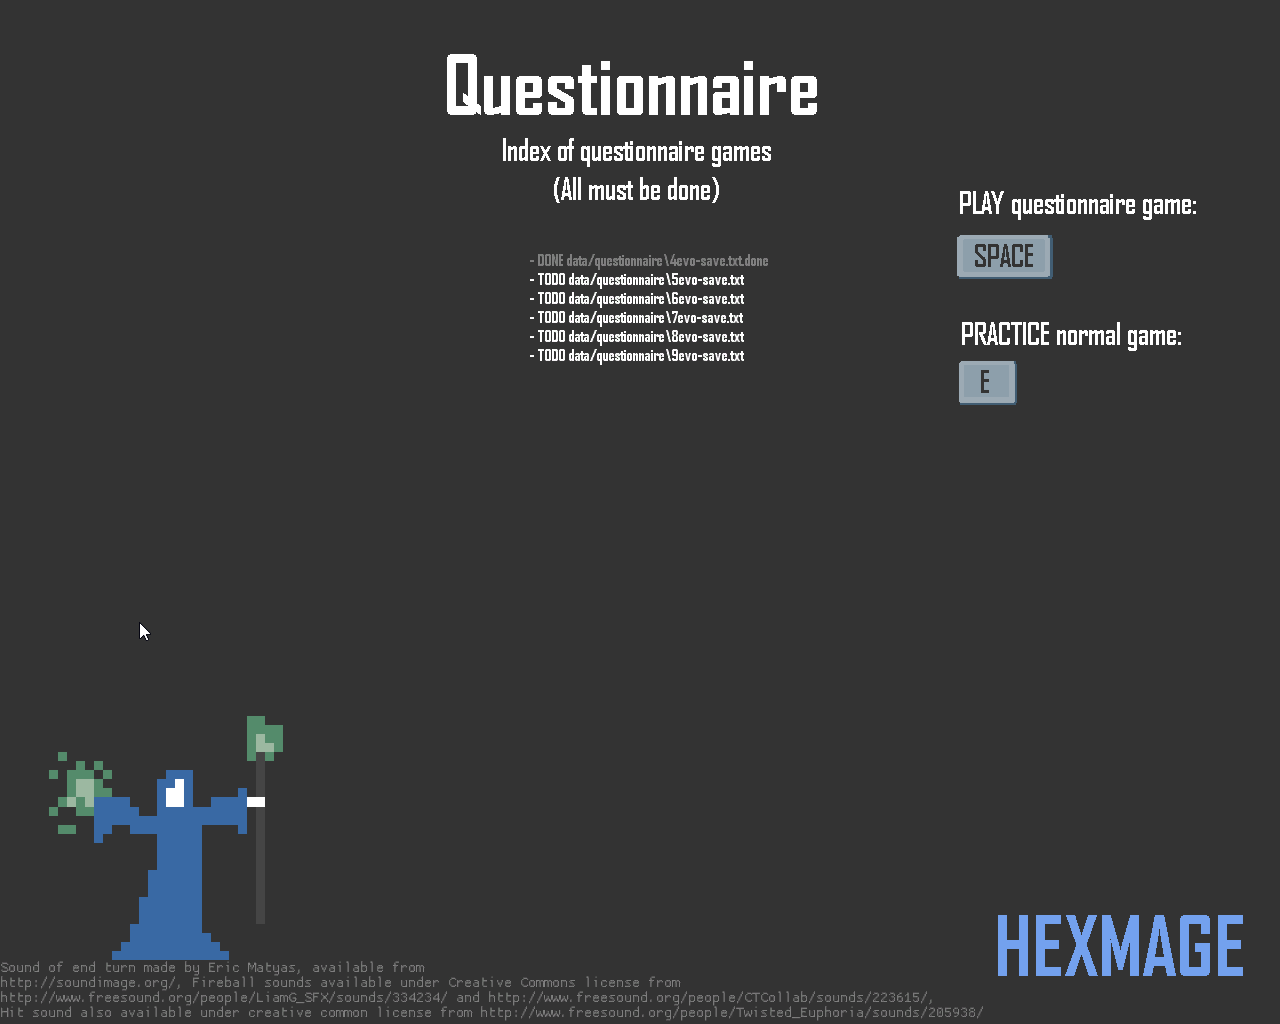
\includegraphics[width=0.95\textwidth]{img/questionnaire.png}
	\label{fig:questionnaire}
	\caption{The main screen of the questionnaire. It shows a list of games which must be played, along with their status. Finished games are displayed in gray and have a \emph{.done} extension, unfinished games are displayed in white. A keyboard shortcut information is also showed.}
\end{figure}

\section{Playing Custom Games}

The user can also press \verb|E| on the initial screen to go into \emph{Practice mode}. This opens up a map editor (see \autoref{fig:map-editor}) where the user can create a custom map, save it to a JSON file (see \autoref{map-format}), load saved files, set startup positions, and continue to the AI selection by pressing \verb|Space|. This allows the user to select AIs for both of the teams and set the team sizes (see \autoref{fig:team-selection}). At any point the user can press \verb|Ctrl-R| to go back to the initial scene. This can be done in game as well.

\begin{figure}
	\centering
	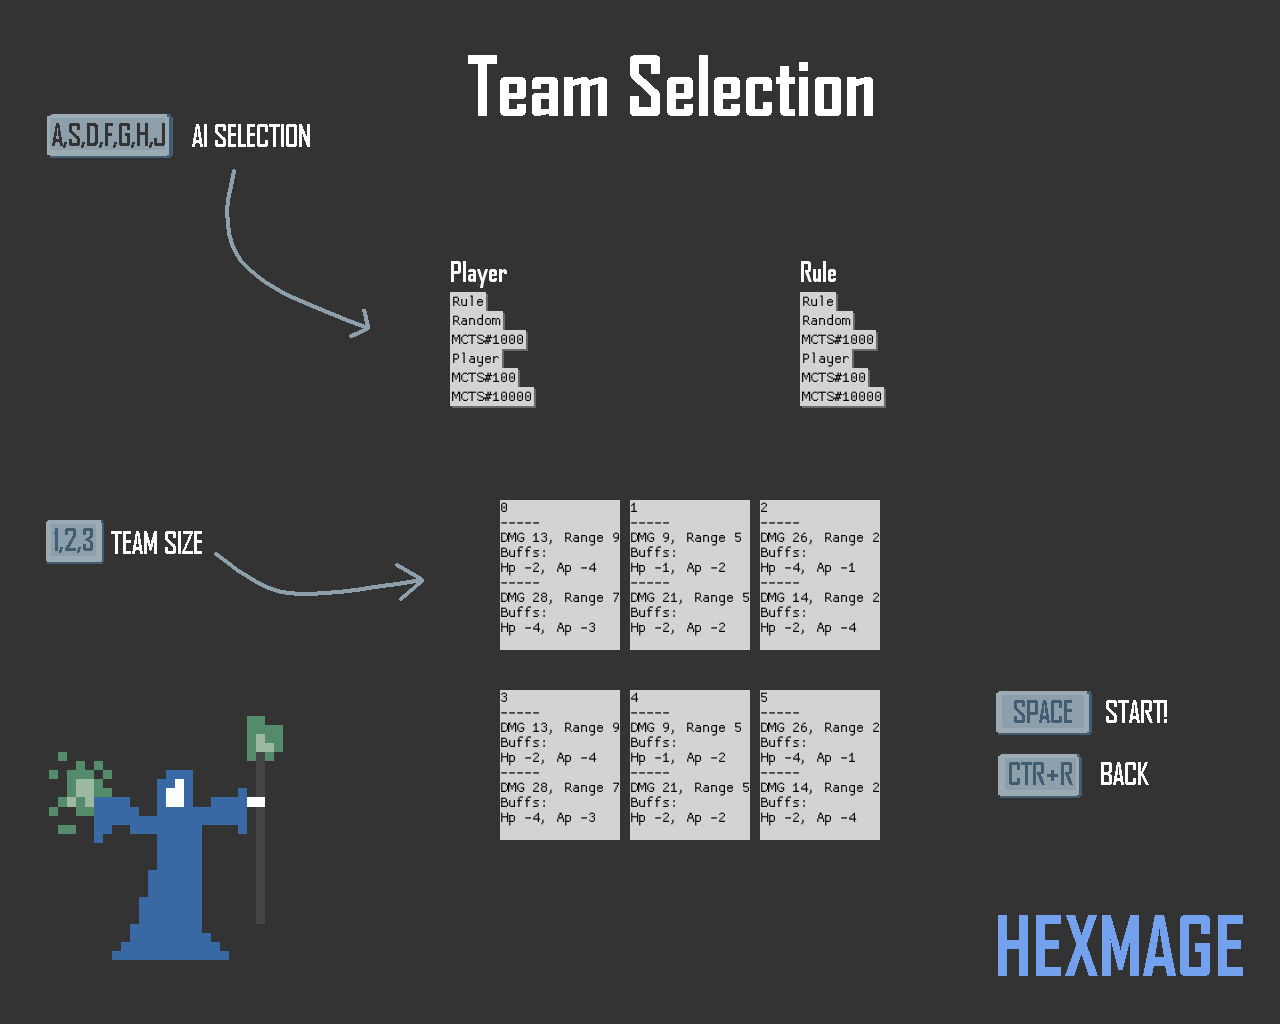
\includegraphics[width=0.95\textwidth]{img/team-selection.png}
	\label{fig:team-selection}
	\caption{Team selection scene which allows the user to pick AIs and team sizes before starting the game. The controls are described on the game screen.}
\end{figure}

Once the user is happy with the team selection, they can press \verb|Space| to start the game, which brings them to the arena scene (see \autoref{fig:arena}). It shows the current game state in the middle of the screen, abilities of the current mage on the left, abilities of the mage under the mouse cursor on the right, the current team at the top, the game history in bottom left, and the detail of a hex under the mouse cursor on the bottom right. Since there is no hidden information, the player can easily see what abilities his opponents have. \autoref{fig:cooldown-no-ap} shows the images representing different ability states. The currently active mage has their underlying hex colored in yellow.

When no ability is selected, the player moves his current mage by clicking the left mouse button on an empty hex. The game displays the distance to the hex in the bottom right corner, as well as drawing the path the mage will walk on. If the target hex is a wall or an enemy is standing on it, the path is not shown, indicating that the mage can not move to the target hex.

Abilities can be selected either by clicking on them with the left mouse button, or with the number keys on the keyboard (\verb|1| for the first, \verb|2| for the second, etc.). When an ability is active, it is shown glowing as shown in \autoref{fig:cooldown-no-ap}. With an active ability, the player can left-click on an enemy mage to use the ability on him. A visiblity indicator is drawn when hovering over an enemy to show whether the enemy is in range and the ability can be used on him.

After the player is finished with his turn, they can press \verb|Space| to finish the turn and move on to the next character.

\begin{figure}
	\centering
	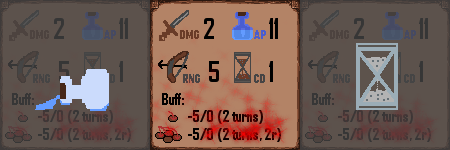
\includegraphics[width=0.60\textwidth]{img/cooldown-no-ap.png}
	\label{fig:cooldown-no-ap}
	\caption{(\emph{Left}) An image shown when the mage does not have enough action points for the given ability. (\emph{Middle}) An image of the currently selected and active ability. (\emph{Right}) An image shown when the given ability is on cooldown.}
\end{figure}
\chapter{Programmer Documentation}
\label{chap:prog-doc}

\section{Used Libraries}
\label{sec:libraries}

While developing desktop GUI applications on Windows provides us with many options, the choices narrow down significantly when the application is a game. As we already established earlier, our choice of language is \Csh{} as it provides the ability to write high level code while maintaining key performance characteristics such as in-place allocated value objects \citep{highperf-dotnet}. Firstly there is Windows Forms \citep{winforms} and Windows Presentation Foundation \citep{wpf} (WPF), which are both excellent desktop GUI libraries, but are not fit for building games as generally require a completely custom user interface. While both Windows Forms and WPF have the ability to embed an OpenGL or DirectX context as a component in their native window components, such approach forfeits all of the benefits of the library and forces the user to implement everything by hand.

Then there is the Unity3D game engine \citep{unity3d} which has a large number of features game developers could need. Unfortunately Unity3D brings its own build system and enforces the developer to structure his game the way Unity3D developers intended. The engine is mostly built for 3D games (with some support for 2D) and as such provides lots of advanced features mainly useful to game developers building larger games. More importantly, Unity3D does not provide any support for tile based movement, hexagonal grids, pathfinding on custom tile-based map, and has a very complicated user interface library tailored mostly for cross platform development. In result, we conclude that using Unity3D would result in us building a lot of things from scratch anyway.

This leaves us with the last contender, which is MonoGame \citep{monogame}, a successor of the previously famous but no longer maintained XNA \citep{xna}. MonoGame is Open Source and available under the Microsoft Public License \citep{ms-pl}. It abstract away the rendering backend and provides a simple API for rendering sprites. It also handles asset packaging (images, sounds, fonts), user input, and provides some basic data structures and algorithms for computer graphics.

We also make use of the Math.NET Numerics \citep{math-dotnet} library for some numerical computation and probability distribution functions, and Newtonsoft Json.NET \citep{json-dotnet} for serialization and deserialization of the JSON files. Both of these can be installed easily via NuGet \citep{nuget} package manager. MonoGame itself needs to be installed with the installer as defined by the instructions on the website \citep{monogame}. Note we only tested with the version 3.5, but newer releases should be compatible as well.

GNU Plot \citep{gnuplot} is also required to generate plots of encounter balancing if the \verb|GnuPlot| constant is set to \verb|true|. It needs to be available in the system \verb|PATH| via \verb|gnuplot.exe| in order to generate the plots (see \verb|GnuPlot.cs| for more details). When the constant is set to \verb|false|, no plots will be generated an the program does not need to be present.

\section{Compilation Instructions}
\label{sec:compilation}

There are two ways to compile our project. First is when one wants to run the \path{HexMage.GUI} project, which requires the libraries specified in \autoref{sec:libraries}. These can be installed via NuGet \citep{nuget}, but one also needs to install MonoGame separately in order to use the MonoGame Pipeline Tool \citep{monogame-pipeline}, which compiles the binary assets under \path{HexMage.GUI/Content} to a binary format which MonoGame can load efficiently. This is not required for compiling and running the \path{HexMage.Benchmarks} project.

After the MonoGame Pipeline Tool is installed, use it to open \path{HexMage.GUI/Content/Content.mcgb} and compile the assets (optionally this could be done through the Visual Studio build system). Next, use NuGet from within Visual Studio 2015 to install the packages. This is done by right-clicking on the \path{HexMage} solution in the \emph{Solution Explorer} and clicking on \emph{Restore NuGet Packages}. Lastly, select the \path{HexMage.GUI} project as a startup project and click the \emph{Run} button. The compilation can also be done from within the \emph{Developer Command Prompt for VS 2015} by going into the root \path{HexMage} directory and running \verb|msbuild HexMage.sln|.

Compiling under Mono is similar, but only works for the \path{HexMage.Benchmarks} and \path{HexMage.Simualtor} projects. First go to the \path{HexMage.Benchmarks} directory and run \verb|nuget restore|. Then, build the project either using the Mono command \verb|xbuild| (or \verb|xbuild /p:Configuration=Release| for a Release build), or if the \verb|make| command is available, you can simply run \verb|make| within the project's directory and it will use its \verb|Makefile| to run \verb|xbuild| automatically.

\section{Constants and Command Line Arguments}
\label{cmd-args}

All of the important constants are configurable through command line arguments, both for the \path{HexMage.Benchmarks} and \path{HexMage.GUI} projects. The constant defaults are configured in \path{Constants.cs}. When the programs are run, the command line arguments are inspected and set respective values in the \path{Constants.cs} class via reflection. Adding a new command line argument is thus as simple as adding a new property to the \path{Constants.cs} file.

The program is then run as following:

\begin{verbatim}
HexMage.Benchmarks.exe --EnableSounds=true \
                       --TeamsPerGeneration=40
\end{verbatim}

will set the \verb|EnableSounds| constant to \verb|true| and \verb|TeamsPerGeneration| to $40$. Constant types are automatically inferred by the reflection mechanism in .NET and can thus be specified without any additional boilerplate. The meaning of each constant is documented in the \path{Constants.cs} file.

\section{Running the Experiments}

There are multiple experiments that can be easily run through the command line via the \path{HexMage.Benchmarks.exe} file (or by running the \path{HexMage.Benchmarks} project in Visual Studio).

The following command line arguments are possible (in addition to the constants defined in \autoref{cmd-args}):

\begin{description}
	\item[mcts-measure-speed] Runs a MCTS speed benchmark which simply generates a random game and keeps playing it over and over again. The main purpose is for running MCTS itself under a profiler.
	
	\item[compare-ai] Runs an AI comparison benchmark. The types of AI that are selected are controlled via the \verb|MctsBenchType| constant (see \autoref{cmd-args}). The selected AIs are run against each other on random games and the resulting win rate is measured.
	
	\item[space-stats] Samples the search space at random points, looks around at neighbours and measures the ratio of upward/downward slopes with their respective fitness change.
\end{description}

When none of these arguments are specified, the encounter balancing algorithm is run on the questionnaire seed data (see \autoref{survey}).

\section{The Game Loop and GameEventHub}

The main game loop in the GUI is represented by a \verb|GameEventHub| class. During each turn, it queries the game state for the current \verb|IMobController| (see \autoref{sec:writing-custom-ai}) and calls its \verb|SlowPlayTurn| method to have the controller execute the turn. After the call returns, the \verb|GameEventHub| automatically ends the turn and moves on to the next character in the turn order.

If the player wishes to pause the game, the \verb|GameEventHub| will delay the game loop until the game is unpaused, which means the game can only be paused at the end of each turn. This however isn't visible to the user, as they can press pause at any time, and if the AI is currently playing, the game will pause once it finishes its turn.

\section{Writing Custom AI}
\label{sec:writing-custom-ai}

The simulator is written in a way which makes it easy to extend it with new AI implementations. One only has to implement the \verb|IMobController| interface. Two methods have to be subclassed:

\begin{description}
	\item[void FastPlayTurn(GameEventHub eventHub)] \hfill \\
	A synchronous implementation of playing a single turn. The \verb|eventHub| object is how the AI author can perform actions in the currently played game. It exposes a method \verb|void FastPlayAction(UctAction action)| which will take an arbitrary action and execute it on the currently played game. Note that instead of passing an \verb|EndTurnAction| the controller should instead return from the \verb|FastPlayTurn| method. It is the responsibility of the caller to end the turn.
	
	\item[Task SlowPlayTurn(GameEventHub eventHub)] \hfill \\
	An asychronous variant of the above function works exactly the same way, except that the caller \verb|await|s on the returned task. It is used in the GUI game loop which executes asynchronously with the main GUI event loop.
\end{description}

Another useful class is \verb|ActionGenerator| which can provide some of the logic behind MCTS and the Rule based AI. Namely the \verb|PossibleActions| generates a list of high level actions which MCTS uses in its decision tree. For more detailed information see the API reference in the attachments. Also see \autoref{sec:invariants} for additional information on how to generate and check the validity of actions.

\section{Creating Encounters with GameInstance}

As described in \autoref{sec:simulator} the \verb|GameInstance| class is the main type in the simulator. It represents the complete encounter together with current game state. Since there are a lot of things that need to be configured, we also provide helpers in the form of \verb|GameSetup| class that can generate a new game with a given map, number of mages, and abilities. 

An important concept we need to describe first is the use of \emph{identifiers} (or handles) throughout the simulator. These are integer types that serve as an identifier of an structure stored and managed internally by the simulator. An example might be using a \verb|int abilityId| parameter instead of a whole \verb|AbilityInfo| class. This allows us to keep the data stored compactly in internal data structures while avoiding unnecessary copying. Since the encounter setup is done only once at the beginning of the game and no abilities/mages are added/removed in the process, we simplified the identifiers to work as indexes directly into the internal array data structures.

While this breaks encapsulation to some extent, it allows us to remove a layer of indirection in the form of lookup tables. An example of this might be accessing a \verb|MobInstance| as \verb|game.State.MobInstances[id]|. A reason for direct array access is that \Csh{} doesn't allow the use of arbitrary references and would introduce unnecessary copying in some cases when the client wants to extract an object, modify it, and store it back. This feature could be handled with a new feature of \Csh{} 7 called \emph{ref return values} \citep{csharp-7} , which allows code to return a reference to a value type from arbitrary functions. However, at the time of writing most of the code \Csh{} 7 was not yet available, which made us stick with the more verbose, yet still functional approach.

It is also worth noting that \verb|GameInstance| and all of its members support shallow and deep copying. A shallow copy can be done by the \verb|CopyStateOnly| method which only makes a copy of the state attributes and thus does not allow the modification of abilities and the map. On the other hand, a deep copy done using \verb|DeepCopy| will copy everything to a new instance and can be used in cases when one wishes to modify the definitions of abilities. This is used when generating the encounters.

\subsection{Encounter Setup}

There are multiple ways one can create an encounter. First we describe all of the necessary structures and how to create them:

\begin{description}
	\item[Map] \hfill \\
	Represents the whole map, can be either created programatically, or loaded from a file using the \verb|Map.Load(string filename)|. Apart from configuring which hexes are walls and which are empty, it is also important to configure the number and positions of starting points for both teams. The game can not be started with a team larger than the number of starting points for that color.
	
	\item[MobManager] \hfill \\
	Keeps all of the immutable information related to the encounter. This consists of \verb|AbilityInfo| and \verb|MobInfo| instances. There is no need to create the \verb|MobManager| manually as the \verb|GameInstance| will take care of it. One can also provide the \verb|GameInstance| with an existing \verb|MobManager| in case it was created beforehand. Such case might be when de-serializing content from a file for example.
	
	\item[AbilityInfo] \hfill \\
	Represents a single ability of a mage. It must be added to the \verb|GameInstance| exclusively through the use of \verb|AddAbilityWithInfo|, since there is an additional internal setup that must be carried out by the \verb|MobManager|.
	
	\item[MobInfo and MobInstance] \hfill \\
	Together these two structures represent a single mage (called \emph{Mob}, short for \emph{mobile object}, internally). \verb|MobInfo| describes the immutable characteristics, such as maximum amount of health and action points, which abilities are available, and the team the mage was assigned to. Note that there is an extra attribute called \emph{initiative} which detemrines a turn order, but was not used in our experiment or encounter generation to simplify the number of variables that needed to be optimized. \verb|MobInfo| objects can be accessed under \verb|game.MobManager.MobInfos|. The \verb|MobInstance| on the other hand contains all of the \emph{current} information, such as current health and action points, position, and debuffs. As such it is stored in the \verb|GameState| object under \verb|game.state.MobInstances|.
\end{description}

Apart from the above mentioned, the \verb|GameState| also holds information about cooldowns and AOEs, and keeps track of the state of the game (whether the game has finished or not).

We also provide a simpler abstractions that are not used directly by the simulator, but store the whole encounter directly and are used in serialization. This is handled mostly by the \verb|GenomeLoader| class together with the \verb|Team| and \verb|DNA| objects. Both \verb|Team| and \verb|DNA| represent the same data but in different format, and can be converted between themselves. If one has already serialized a setup and loaded it with the \verb|JsonLoader| object, it can be then converted directly into a \verb|GameInstance| using \verb|GameSetup.UnpackTeamsIntoGame| method (see API documentation for details). Another good reference can be both the \verb|AiRandomController| and \verb|AiRuleBasedController| which are both rather simple and contain only the necessary boilerplate to get things working.

\subsection{Invariants and Action Validation}
\label{sec:invariants}

Since our game mechanics are rather complicated, we provide a set of runtime checks that verify most of the game mechanics. These can be found under \verb|GameInvariants| and are mostly turned on only when the \verb|DEBUG| compile constant is defined. This is done automatically when doing a Debug build in Visual Studio, and is automatically turned off in Release mode. We made these checks conditional since they can be rather expensive and slow down the simulation a lot.

The class also provides some predicates which are not debug-only and are used by the simulator to check if a given action is valid. For example, one can check if an ability can be used on a target with the \verb|IsAbilityUsable| method. This will check if the target is an enemy, alivem, visible from our current position, if we have enough action points, if the ability is not on cooldown and if the target is within range. These helpers can also serve the programmer developing an AI for our game, as all of the game logic has been encapsulated and the programmer can simply check if some action is valid, without having to implement all of the game rules themself.

\section{Extending the Game UI}

The UI is structured as a tree of \verb|Entity| objects, each with a number of attached \verb|Component| instances. Each \verb|Entity| has an information about its position and a parent relationship. It can also optionally have a \verb|Renderer| attached (subclass of the \verb|IRenderer| interface), which takes care of the actual rendering. The \verb|IRenderer| has a simple interface that only requires implementing a \verb|Render| method, which can do any arbitrary rendering using the MonoGame \citep{monogame} API.

\subsection{Entities and Components}

A new \verb|Component| can be either created by sub-classing, or by using a shorthand with the \verb|LambdaComponent| class, which allows components to be defined simply by their \verb|Update| method provided as a lambda function. There are no restrictions on the \verb|Update| function, except for deleting entities. This must be done by the use of the scene's \verb|DestroyEntity| method which will queue up the delete until a next frame update. The reason is that we can't know if the deleted entity still needs its components to be updated within the current frame, or if they were already updated, or if we are actually deleting the parent of the current entity.

We also provide two additional helpers for delaying actions. Firstly, there is \verb|AfterUpdate| which takes an arbitrary action and runs it after all of the \verb|Update| functions have been called. And then there is also \verb|DelayFor|, which works similarly but also takes a time for which the action should be delayed. The time keeping is managed automatically by the \verb|GameScene|.

Similarly, newly added entities need to be initialized, and as such one should always use the \verb|AddAndInitializeRootEntity| when adding a root entity. Child entities are initialized automatically by their parents. This leads us to the component and entity lifecycle. First each entity is initialized with their respective \verb|Initialize| method, then each root entity has its \verb|Layout| method called (and recursively calls down to children automatically), then all root entities have their \verb|Update| method called, and lastly, all entities which have a \verb|IRenderer| attached have their \verb|Render| methods called. During the \verb|Update| call, the \verb|GameScene| will also automatically call \verb|Update| on the entitie's components.

\subsection{Scenes}

Each screen in the game is represented by a \verb|GameScene| object. These objects are automatically managed by the \verb|SceneManager| which keeps a stack of scenes and executes the lifecycle loop on the currently top scene. Scenes can terminate themselves using the \verb|Terminate| call which will destroy the scene at the end of its event loop, and new scenes can be added using \verb|LoadNewScene|.

\openright
\end{document}
